\documentclass{article}
\usepackage[utf8]{inputenc}

\usepackage[plain]{fullpage}

\usepackage{natbib}
\usepackage{graphicx}

\usepackage{hyperref}

\usepackage{amsthm}
\usepackage{amssymb}


\newtheorem{theorem}{Theorem}
\newtheorem{lemma}{Lemma}
\newtheorem{corollary}{Corollary}
\newtheorem{property}{Property}
\newtheorem{proposition}{Proposition}
\newtheorem{fact}{Fact}


% TikZ ---------------------------------------------
\usepackage{tikz}
\usetikzlibrary{calc}
\usetikzlibrary{snakes}
\usetikzlibrary{trees}
\tikzstyle{vertex}=[circle,fill=black!0,minimum size=4pt,inner sep=0pt]
\tikzstyle{smallvertex}=[circle,fill=black!0,minimum size=3pt,inner sep=0pt]

\usepackage{cleveref} % MUST BE LOADED LAST


\title{Lecture Notes - Advanced Algorithms for Data Science}
\author{Scribe: Firstname \textsc{Lastname} - Lecture by Gregory \textsc{Kucherov}}
\date{2016-XX-XX - Part XX}

\begin{document}

\maketitle

\section{About the script}

This file will be used as part of your grade
for this course: every student is supposed to edit
lecture notes for one hour of the course.

\subsection{How to write the script}

The script should be written into Section~\ref{yourSection}
below (entitled ``Your section''). They should be written in english. 
They should be clear and easy to read, e.g. by other students. 
Do not hesitate to add examples (other
than the ones presented at the lecture) and figures.
For the figures, two examples written in ``TikZ'' are
given below (see Figure~\ref{fig:TCBLglobal})
in case you are not familiar with this language.

The script should include appropriate bibliographical
references to the cited theorems and algorithms,
and should mention the source for the figures or paragraphs
copied from other documents.
We expect the script to be at least 3 pages long, but they should not
exceed 10 pages. 

\subsection{Write more than just the lecture}

In your notes you should write down full details of the proofs of the statements
(theorems, lemmas, algorithm correctness, \ldots) made in the
lecture. For that, you may have to consult some textbooks or other
sources. Please contact the professor if you need more information
about bibliographic references. 

It is important that you provide a comprehensive insight into the
material. The minimum requirement is to provide a complete account of
the material presented at the lecture, however {\bf it is very desirable
that you extend it with some other results} such as interesting
special cases, or variants of the result, or examples of
application, etc. Again, contact the professor if you have doubts
about incuding some material. 

\subsection{Submitting the script}

You have to submit your script to {\sc Moodle}, together with
necessary supplementary files (.bib, figures). {\bf The deadline is
November 27, however you are strongly advised to write your script
shortly after the corresponding lecture.} 

\subsection{Evaluation}

Here are the criteria that will be used to grade
your script:
\begin{itemize}
\setlength{\itemsep}{0mm}
\item Content: comprehensive, extended material provided
\item Content: correct and mathematically rigorous
\item Content: clearly written
\item Style: well-illustrated 
\item Style: clean and well-structured
\item Style: respecting all constraints on number of pages, file names, etc.
\item Style: english writing \& spelling
\item Style: bibliography
\end{itemize}
 

\section{Your section}\label{yourSection}

Please put all your content in this section. Don't
forget to add bibliographic references as well,
in the file \texttt{references.bib}.

\subsection{First subsection}

``I always thought something was fundamentally wrong with the universe'' \citep{adams1995hitchhiker}. 
There is a nice picture of the universe
in Figure~\ref{fig:universe}.

\begin{figure}[h!]
\centering
\includegraphics[scale=1.7]{Lastname_universe.jpg}
\caption{The Universe}
\label{fig:universe}
\end{figure}

\subsection{Second subsection}

There is a nice figure with a tree and a network
in Figure~\ref{fig:TCBLglobal}.
\begin{figure}[gt]
\centering
\begin{tabular}{ccc}
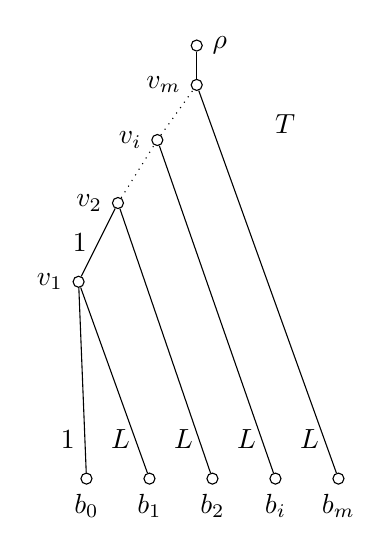
\begin{tikzpicture}
% vertices
\node[vertex,draw] (rootparent) at (3,5.5) [label=right:$\rho$] {};
\node[vertex,draw] (root) at (3,5) [label=left:$v_m$] {};
\node[vertex,draw] (v3) at (2.5,4.3) [label=left:$v_i$] {};
\node[vertex,draw] (v2) at (2,3.5) [label=left:$v_2$] {};
\node[vertex,draw] (v1) at (1.5,2.5) [label=left:$v_1$] {};
\node[vertex,draw] (b0) at (1.6,0) [label=below:$b_{0}$] {};
\node[vertex,draw] (b1) at (2.4,0) [label=below:$b_1$] {};
\node[vertex,draw] (b2) at (3.2,0) [label=below:$b_2$] {};
\node[vertex,draw] (b3) at (4,0) [label=below:$b_i$] {};
\node[vertex,draw] (b4) at (4.8,0) [label=below:$b_m$] {};

\node (v12) at (1.85,3) [label=left:1] {};
\node (v10) at (1.7,0.5) [label=left:1] {};
\node (vb1) at (2.4,0.5) [label=left:$L$] {};
\node (vb2) at (3.2,0.5) [label=left:$L$] {};
\node (vbi) at (4,0.5) [label=left:$L$] {};
\node (vbm) at (4.8,0.5) [label=left:$L$] {};
\node (T) at (4.5,4.5) [label=left:$T$] {};

% edges and paths
\draw (rootparent) -- (root);
\draw (v1) -- (v2);
\draw [dotted] (v2) -- (v3);
\draw [dotted] (v3) -- (root);
\draw (b0) -- (v1);
\draw (b1) -- (v1);
\draw (b2) -- (v2);
\draw (b3) -- (v3);
\draw (b4) -- (root);
\end{tikzpicture}
& ~ &
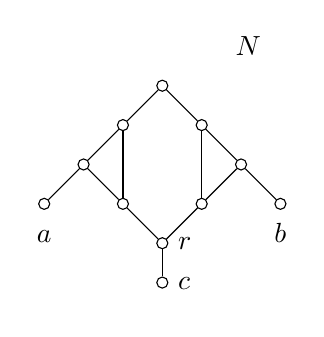
\begin{tikzpicture}
% vertices
\node[vertex,draw] (root) at (0,2) {};

\node[vertex,draw] (app) at (-0.5,1.5) {};
\node[vertex,draw] (bpp) at (0.5,1.5) {};

\node[vertex,draw] (ap) at (-1,1) {};
\node[vertex,draw] (dp) at (1,1) {};

\node[vertex,draw] (a) at (-1.5,0.5) [label=below:$\strut a$] {};
\node[vertex,draw] (b) at (1.5,0.5) [label=below:$\strut b$] {};
\node[vertex,draw] (as) at (-0.5,0.5) {};
\node[vertex,draw] (bs) at (0.5,0.5) {};
\node[vertex,draw] (r) at (0,0) [label=right:$\strut r$] {};

\node[vertex,draw] (c) at (0,-0.5) [label=right:$\strut c$] {};

% unlabelled vertices

% edges and paths
\draw (root) -- (app);
\draw (root) -- (bpp);
\draw (app) -- (ap);
\draw (bpp) -- (dp);
\draw (bpp) -- (bs);
\draw (app) -- (as);

\draw (a) -- (ap);
\draw (as) -- (ap);
\draw (r) -- (c);
\draw (bs) -- (dp);
\draw (b) -- (dp);

\draw (as) -- (r);
\draw (r) -- (c);
\draw (bs) -- (r);

\node (N) at (1.5,2.5) [label=left:$N$] {};

\end{tikzpicture}

\end{tabular}
\caption{An illustration of a tree $T$ and a network $N$
.}
\label{fig:TCBLglobal}
\end{figure}

\bibliographystyle{plain}
\bibliography{references}
\end{document}
